\documentclass{article}
    \usepackage{graphicx} % Used to insert images
    \usepackage{adjustbox} % Used to constrain images to a maximum size 
    \usepackage{color} % Allow colors to be defined
    \usepackage{enumerate} % Needed for markdown enumerations to work
    \usepackage{geometry} % Used to adjust the document margins
    \usepackage{amsmath} % Equations
    \usepackage{amssymb} % Equations
    \usepackage[mathletters]{ucs} % Extended unicode (utf-8) support
    \usepackage[utf8x]{inputenc} % Allow utf-8 characters in the tex document
    \usepackage{fancyvrb} % verbatim replacement that allows latex
    \usepackage{grffile} % extends the file name processing of package graphics 
                         % to support a larger range 
    % The hyperref package gives us a pdf with properly built
    % internal navigation ('pdf bookmarks' for the table of contents,
    % internal cross-reference links, web links for URLs, etc.)
    \usepackage{hyperref}
    \usepackage{longtable} % longtable support required by pandoc >1.10
    \usepackage{booktabs}  % table support for pandoc > 1.12.2
    % Math Jax compatability definitions
    \def\gt{>}
    \def\lt{<}
    
	\author{Jonas Kersulis}
	\title{Transmission line temperature modeling}
	\date{ }
	
    \begin{document}
    
    \maketitle
    
\begin{abstract}
This document derives an approximate line temperature equation that is second-order in angle difference. This makes it compatible with the temporal instanton optimization formulation. Numerical experimentation indicates that the derived equation matches the IEEE 738 standard closely, and where the two models differ, the approximate equation is conservative.
\end{abstract}
    
\section{Approximate line temperature equation}\label{transmission-line-heating}

\subsection{The heat balance equation}
    The change in temperature of any object may be expressed as a
differential equation. This equation, called the heat balance equation,
relates change in temperature to a sum of various sources of heating.
For a transmission line, these sources are:

\begin{enumerate}
\item
  Resistive heating, also known as $I^2R$ losses. This heat source is a
  function of power flow on the line. In general, the line's resistance
  varies with temperature, making this calculation more complicated than
  it appears.
\item
  Convective heating, which is directly proportional to the temperature
  difference between the line and the surrounding air. If the line is
  hotter than the surrounding air, it will ``give off heat'' via
  convection -- particles moving away from the line will carry energy
  with them.
\item
  Radiative heating. This heating is related to line and ambient
  temperatures raised to the fourth power. Physically, thermal radiation
  is the process by which thermal energy is converted to electromagnetic
  energy. It takes place in all objects whose absolute temperature is
  greater than zero.
\item
  Solar irradiation. The sun imparts energy to the transmission line
  according. The magnitude of this energy transfer is a function of
  clouds, geometry, and the line's insulation material. Reflective
  insulation admits very little solar energy, while black insulation
  results in significant solar thermal heating.
\end{enumerate}

    These heat sources are summed together in the heat balance equation,
which tells us how quickly (and in what direction) the transmission
line's temperature will change:

\begin{align}\label{eq:heatbalance}
\frac{dT}{dt} &= \frac{1}{m\cdot C_p}\left[I^2\cdot R(T) - q_c - q_r + q_s \right]
\end{align}

In this equation, $T$ is the conductor average temperature, $I^2\cdot R(T)$ represents line losses, $q_c$ is the convective heat rate, $q_r$ is the radiative heat rate, and $q_s$ is the solar heat rate.

\begin{enumerate}
\item
  In the temporal instanton setting, $I^2\cdot R(T)$ is replaced by
  $f_{ij}^\text{loss}$, the DC approximate line losses.
\item
  The convection heat rate is expressed as
  \begin{align}\label{eq:qc}
  \eta_c\cdot(T - T_\text{amb})~,
  \end{align}
  where $T_\text{amb}$ is the ambient temperature (of surrounding air).
\item
  The radiation heat rate is given by
  \begin{align}\label{eq:qr}
    \eta_r\cdot\left[(T + 273)^4 - (T_\text{amb} + 273)^4\right]
  \end{align}
\item
  The solar heat rate is fixed to some conservative constant (representing full direct sun, for example).
\end{enumerate}

\subsection{Linearization of radiation heat rate}

    When \eqref{eq:heatbalance} is combined with a given initial temperature $T_0$, the
resulting initial value problem makes it possible to determine the temperature at some later time. Let's substitute the DC loss approximation, \eqref{eq:qc}, and \eqref{eq:qr} into \eqref{eq:heatbalance} and attempt to solve for temperature:

\begin{align}
\frac{dT}{dt} &= \frac{1}{mC_p}\left[ f_{ij}^\text{loss} - \eta_c\left( T(t) - T_\text{amb}\right) - \eta_r\left((T(t) + 273)^4 - (T_\text{amb} + 273)^4\right) + q_s \right]
\end{align}

Suppose that power flow, ambient temperature, and solar heat rate are constant during the temperature change calculation. Then there are only two variable terms on the right-hand side: one first-order, one fourth-order. The fourth-order term (which corresponds to radiation) makes this equation difficult to solve. Fortunately, this term is approximately linear over the temperature range we are interested in. The figure below shows how we might linearize the radiation heat rate conservatively\footnote{Because a transmission line is typically at a higher temperature than surrounding air, radiation tends to decrease line temperature. Thus, a conservative approach will underestimate the radiation heat rate, leading to slightly higher temperatures.}.

\begin{figure}[h]
\centering
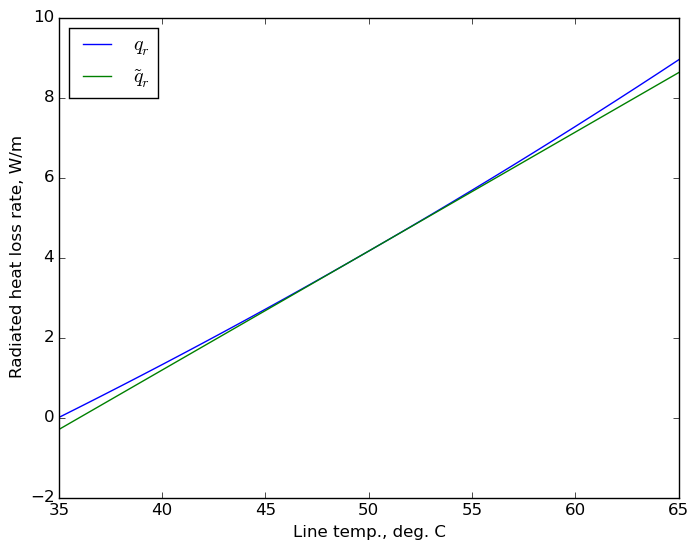
\includegraphics[width=0.7\linewidth]{../images/rad_approx}
\caption{Comparison of fourth-order radiation heat rate \eqref{eq:qr} with a conservative linearization across a range of temperatures. Note that the ambient temperature is 35$^\circ$C.}
\label{fig:rad_approx}
\end{figure}

The green trace is the linearization of $q_r$ about $T_\text{mid}$, the midpoint between the ambient and limit temperatures. Let's replace $q_r$ by this linear approximation $\tilde{q}_r$:

\begin{align}\label{eq:approx_qr}
\frac{dT}{dt} &= \frac{1}{mC_p}\left[ f_{ij}^\text{loss} - \eta_c\left( T(t) - T_\text{amb}\right) - \tilde{q}_r + q_s \right]
\end{align}

where

\begin{align}
\tilde{q}_r &= \eta_r  \left( (T_\text{mid} + 273)^4 - (T_\text{amb} + 273)^4\right) + 4\eta_r(T_\text{mid} + 273)^3\cdot(T(t) - T_\text{mid})
\end{align}


\subsection{Line temperature as IVP solution}
After simplification, \eqref{eq:approx_qr} becomes

\begin{align}\label{eq:diffeq}
\frac{dT}{dt} &= aT(t) + b
\end{align}

where constants $a$ and $b$ are defined as

\begin{subequations}
\begin{align}
a &= \frac{1}{mC_p} \left[ -\eta_c - 4\eta_r(T_\text{mid} + 273)^3 \right] \\
b &= \frac{1}{mC_p} \left[ f_{ij}^\text{loss} + \eta_cT_\text{amb} - \eta_r \left( (T_\text{mid} + 273)^4 - (T_\text{amb} + 273)^4 \right) + 4\eta_rT_\text{mid}(T_\text{mid} + 273)^3 + q_s \right]
\end{align}
\end{subequations}

The differential equation \eqref{eq:diffeq} has a straightforward solution:

\begin{align}\label{eq:tivp}
T(t) &= ke^{at} - \frac{b}{a}
\end{align}

where $k=T(0) + b/a$. Note that $b$ is influenced by power flow (via
$f_{ij}^\text{loss}$), but $a$ is not.

%    \section{Line temperature simulation}\label{line-temperature-simulation}
%
%Suppose we want to track line temperature over the course of 30 minutes,
%and we are able to update power flow information every 10 minutes. Each
%time the angle difference across the line changes, so do
%DC-approximate losses. When losses change, the constants $b$ and $k$
%change in the temperature equation. The final temperature of
%each 10-minute interval becomes the initial temperature of the
%next interval.
%
%The following figure is a plot of temperature versus time for a single
%transmission line. The line's parameters were chosen according to
%typical RTS-96 values. The three sliders represent angle difference (in
%radians) across the line during each 10-minute interval. The angle
%difference is large enough during the first interval to cause the line
%to heat up, but small enough in the second interval to allow it to cool
%down. The angle difference in the third interval is large enough to
%drive the line to its temperature limit (horizontal red line) by the
%last time step.
%
%\begin{figure}[h]
%\centering
%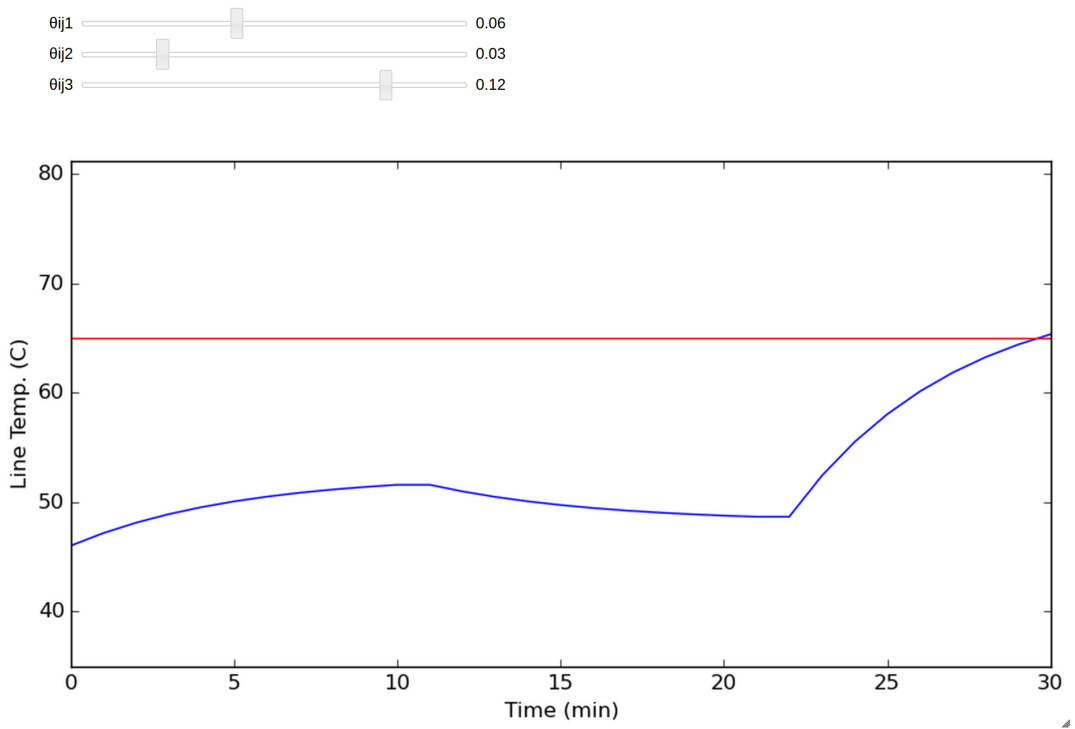
\includegraphics[width=\linewidth]{../images/multi-step-heating}
%\caption{Tracking line temperature across three ten-minute time intervals, with different power flow during each interval}
%\label{fig:multi-step-heating}
%\end{figure}
%    
    

\section{From temperature equation to optimization
constraint}\label{from-ivp-to-optimization-constraint}

The important thing to note about the temperature equation \eqref{eq:tivp} is that it is influenced only by initial temperature and the angle difference during each time interval. There is therefore a recursive relationship between final temperature and initial temperature that involves only angle differences.

\subsection{Recursive relationship between final and initial temperatures}
Suppose there are three time intervals: $t_1$, $t_2$, and $t_3$. Then the line temperature at the end of the third interval is given by

\begin{align}
\nonumber T(t_3) &= k_3 e^{(t_3-t_2)a} - \frac{b_3}{a} \\
\nonumber &= \left[k_2 e^{(t_2-t_1)a} - \frac{b_2}{a} + \frac{b_3}{a}\right]e^{(t_3-t_2)a} - \frac{b_3}{a} \\
\nonumber &= \left[\left( T(t_1) + \frac{b_2}{a} \right)e^{(t_2-t_1)a} - \frac{b_2}{a} + \frac{b_3}{a}\right]e^{(t_3-t_2)a} - \frac{b_3}{a} \\
\label{eq:Texpand} &= \left\lbrace\left[\left(T(t_0) + \frac{b_1}{a}\right) e^{(t_1-t_0)a} - \frac{b_1}{a} + \frac{b_2}{a}\right]e^{(t_2-t_1)a} - \frac{b_2}{a} + \frac{b_3}{a}\right\rbrace e^{(t_3-t_2)a} - \frac{b_3}{a}
\end{align}
The recursive pattern is apparent. Because all time intervals are the same length, we have
\begin{align*}
e^{(t_3-t_2)a} &= e^{(t_2-t_1)a} = e^{(t_1-t_0)a}~,
\end{align*}
and we can distribute in \eqref{eq:Texpand} to obtain
\begin{align}
T(t_3) &= (e^{(t_1-t_0)a})^3\left(T(t_0) + \frac{b_1}{a}\right) + (e^{(t_1-t_0)a})^2\left(- \frac{b_1}{a} + \frac{b_2}{a}\right) + (e^{(t_1-t_0)a})\left(- \frac{b_2}{a} + \frac{b_3}{a}\right) - \frac{b_3}{a}
\end{align}
Because power flow data enters through $b_1$, $b_2$, and $b_3$, it makes sense to
group terms accordingly:

\begin{multline}
T(t_3) = ((e^{(t_1-t_0)a})^3T(t_0) + \left(\frac{(e^{(t_1-t_0)a})^3}{a} - \frac{(e^{(t_1-t_0)a})^2}{a}\right)b_1 + \\ + \left( \frac{(e^{(t_1-t_0)a})^2}{a} - \frac{(e^{(t_1-t_0)a})^1}{a}\right)b_2 + \left(\frac{e^{(t_1-t_0)a}}{a} - \frac{1}{a}\right) b_3
\end{multline}
The pattern in the above expression makes it easy to extend $T(t_3)$ to cover the general case $T(t_n)$:

\begin{align}\label{eq:recursive}
T(t_n) &= (e^{(t_1 - t_0)a})^n T(t_0) + \frac{1}{a} \sum_{i=1}^n \left( (e^{(t_1-t_0)a})^i - (e^{(t_1-t_0)a})^{i-1} \right)b_{n-i+1}
\end{align}

Ultimately \eqref{eq:recursive} will be used to constrain a line's final temperature to some limiting value. The remainder of this section will relate \eqref{eq:recursive} back to power flow angles so it can be ``plugged in'' to the optimization framework.

\subsection{Relating temperature to angle differences}

Recall that $b_n$ depends on the angle difference at time $t_n$:

\begin{align}
\nonumber b_n &= \frac{1}{mC_p} \left[ \frac{r_{ij}}{x_{ij}^2}\cdot \frac{S_b}{3L_{ij}} \theta_{ij}(t_n)^2 + \eta_cT_\text{amb} - \eta_r\left((T_\text{mid} + 273)^4 - (T_\text{amb} + 273)^4\right) + 4\eta_rT_\text{mid}(T_\text{mid} + 273)^3 + q_s \right] \\
\label{eq:bexpand} b_n &= c\theta_{ij}(t_n)^2 + d
\end{align}
where constants $c$ and $d$ are defined as:
\begin{align*}
c &= \frac{r_{ij}S_b}{3 mC_p x_{ij}^2L_{ij}} \\
 d &= \frac{1}{mC_p}\left[ \eta_cT_\text{amb} - \eta_r\left((T_\text{mid} + 273)^4 - (T_\text{amb} + 273)^4\right) + 4\eta_rT_\text{mid}(T_\text{mid} + 273)^3 + q_s \right]
\end{align*}
Substitute \eqref{eq:bexpand} into \eqref{eq:recursive}:
\begin{align*}
T(t_n) &= (e^{(t_1 - t_0)a})^n T(t_0) + \frac{1}{a} \sum_{i=1}^n \left( (e^{(t_1-t_0)a})^i - (e^{(t_1-t_0)a})^{i-1} \right)(c\theta_{ij}(t_{n-i+1})^2 + d)
\end{align*}
Expand the sum term:
\begin{multline}\label{eq:sumexpand}
\frac{1}{a} \sum_{i=1}^n \left( (e^{(t_1-t_0)a})^i - (e^{(t_1-t_0)a})^{i-1} \right)(c\theta_{ij}(t_{n-i+1})^2 + d) = \frac{c}{a}\left[ \sum_{i=1}^n \left( (e^{(t_1-t_0)a})^i - (e^{(t_1-t_0)a})^{i-1} \right)\theta_{ij}(t_{n-i+1})^2\right] + \\  \qquad + \frac{d}{a}\left[ \sum_{i=1}^n \left( (e^{(t_1-t_0)a})^i - (e^{(t_1-t_0)a})^{i-1} \right)\right] 
\end{multline}
Substitute \eqref{eq:sumexpand} into the line temperature equation, introducing the constant $f$ to keep things a bit neater:
\begin{align}\label{eq:almostthere}
T(t_n) &= f + \frac{c}{a}\left[ \sum_{i=1}^n \left( (e^{(t_1-t_0)a})^i - (e^{(t_1-t_0)a})^{i-1} \right)\theta_{ij}(t_{n-i+1})^2\right]
\end{align}
where
\begin{align}
f &= (e^{(t_1 - t_0)a})^n T(t_0) + \frac{d}{a}\left[ \sum_{i=1}^n \left( (e^{(t_1-t_0)a})^i - (e^{(t_1-t_0)a})^{i-1} \right)\right]
\end{align}
Rearrange \eqref{eq:almostthere} to isolate angle differences:
\begin{align}
\sum_{i=1}^n \left( (e^{(t_1-t_0)a})^i - (e^{(t_1-t_0)a})^{i-1} \right)\theta_{ij}(t_{n-i+1})^2 &= \frac{a}{c}(T(t_n) - f)
\end{align}
Now define
\begin{equation}\label{eq:thetahat}
\hat{\theta}_{ij}(t_{k})=  \theta_{ij}(t_k)\sqrt{ (e^{(t_1-t_0)a})^{n-k+1} - (e^{(t_1-t_0)a})^{n-k} }
\end{equation}
to obtain
\begin{align}\label{eq:finaltemp}
\sum_{k=1}^n \hat{\theta}_{ij}(t_{k})^2 &= \frac{a}{c}\left(T(t_n) - f\right)
\end{align}
The expression \eqref{eq:finaltemp} may be used to constrain line temperature to be equal to some limiting value by the end of the last time interval.

This derivation has been somewhat messy. The line temperature constraint is summarized in the next section for convenience.

\subsection{Summary of line temperature
constraint}\label{summary-of-line-temperature-constraint}

Suppose our time horizon consists of $n$ intervals, each on the order of
ten minutes long. Power flow data is updated after each interval, but
all other parameters remain constant. Choose a single transmission
line in the network, and suppose it lies between nodes $i$ and $j$. This line has a
thermal limit of $T_\text{lim}$ ($^\circ$C). We can constrain the
line's temperature to be equal to this limiting value by enforcing the
second-order constraint:

\begin{align}\label{eq:tempconstraint}
\sum_{k=1}^n \hat{\theta}_{ij}(t_k)^2 &= \frac{a}{c}\left(T_\text{lim} - f\right)
\end{align}

where

\begin{itemize}
\itemsep1pt\parskip0pt\parsep0pt
\item
  $\hat{\theta}_{ij}(t_{k})=  \theta_{ij}(t_k)\sqrt{ (e^{(t_1-t_0)a})^{n-k+1} - (e^{(t_1-t_0)a})^{n-k} } $

  \begin{itemize}
  \itemsep1pt\parskip0pt\parsep0pt
  \item
    $\theta_{ij}(t_k)$ is the angle difference across line $ij$ at time
    interval $t_k$.
  \item
    $(t_1-t_0)$ is the length of each time interval (in seconds)
  \end{itemize}
\item
  $ a =
  \frac{1}{mC_p}\left[ -\eta_c - 4\eta_r(T_\text{mid} + 273)^3 \right]$
  is constant with units of $s^{-1}$

  \begin{itemize}
  \itemsep1pt\parskip0pt\parsep0pt
  \item
    $mC_p$ is the heat capacity, with units of J/m-$^\circ$C
  \item
    $\eta_c$ is the conductive heat loss rate coefficient, with units of
    W/m-$^\circ$C
  \item
    $\eta_r$ is the conductive heat loss rate coefficient, with units of
    W/m-$^\circ$C$^4$
  \item
    $T_\text{mid}$ is the average of ambient temperature $T_\text{amb}$
    and limit temperature $T_\text{lim}$, in Celsius
  \end{itemize}
\item
  $c = \frac{r_{ij}S_b}{3 mC_p x_{ij}^2L_{ij}}$ is a constant with units
  of W/m

  \begin{itemize}
  \itemsep1pt\parskip0pt\parsep0pt
  \item
    $r_{ij}$ is resistance of line $ij$ in per unit
  \item
    $x_{ij}$ is reactance of line $ij$ in per unit
  \item
    $S_b$ is the system base (e.g.~100 MVA)
  \item
    $L_{ij}$ is the length of one phase of line $ij$, in m
  \end{itemize}
\item
  $f = (e^{(t_1 - t_0)a})^n T(t_0) + \frac{d}{a}\left[ \sum_{i=1}^n \left( (e^{(t_1-t_0)a})^i - (e^{(t_1-t_0)a})^{i-1} \right)\right]$
  is a constant with units of degrees Celsius

  \begin{itemize}
  \itemsep1pt\parskip0pt\parsep0pt
  \item
    $T(t_0)$ is the line's initial temperature (steady state temperature
    under base case power flow condition)
  \item
    $d = \frac{1}{mC_p}\left[ \eta_cT_\text{amb} - \eta_r\left((T_\text{mid} + 273)^4 - (T_\text{amb} + 273)^4\right) + 4\eta_rT_\text{mid}(T_\text{mid} + 273)^3 + q_s \right]$
    is a constant with units of W/m

    \begin{itemize}
    \itemsep1pt\parskip0pt\parsep0pt
    \item
      $q_s$ is the solar heat gain rate in W/m
    \end{itemize}
  \end{itemize}
\end{itemize}



\section{Numerical comparison to IEEE 738 standard model}\label{numerical-comparison-of-temperature-models}

To validate the approximate line temperature model derived here, I compared it to the IEEE 738 standard model using RTS-96 and Waxwing conductor parameters.

\subsection{Summary of IEEE 738 temperature
calculation}\label{summary-of-ieee-738-temperature-calculation}

IEEE recommends numerically integrating \eqref{eq:heatbalance} to compute temperature changes. The temporal instanton framework uses approximate DC losses in place of $I^2R(T_\text{avg})$, so we will be integrating the following heat balance equation:

\begin{align}\label{eq:738heatbalance}
\frac{dT_\text{avg}}{dt} &= \frac{1}{mC_p}\left( r_{ij}\frac{\theta_{ij}^2}{x_{ij}^2}\frac{S_b}{3L_{ij}} - q_c - q_r + q_s\right)
\end{align}

Heat rates $q_c$ and $q_r$ are calculated according to \eqref{eq:qc} and \eqref{eq:qr}, respectively (copied here for convenience):
\begin{align*}
q_c &= \eta_c\cdot(T - T_\text{amb}) \\
q_r &= \eta_r\cdot((T + 273)^4 - (T_\text{amb} + 273)^4)
\end{align*}
All other parameters are constant during temperature calculation. The important thing to keep in mind about IEEE 738 temperature calculation is that it requires numerical integration; there is no analytic temperature solution for \eqref{eq:738heatbalance}. This means one must select an integration time step $\Delta t$. For each step, one computes the change in temperature by multiplying $\Delta t$ by the value of \eqref{eq:738heatbalance} computed at that step. IEEE recommends a step size smaller than 10\% of the conductor thermal time constant\footnote{A typical transmission line thermal time constant is ten minutes, which means IEEE recommends an integration step size of one minute}. A smaller integration step size yields more accurate results.

\subsection{Comparison}\label{comparison}

I used RTS-96 network data and Waxwing conductor parameters to compare IEEE 738 standard temperature calculation to the model derived in Section \ref{transmission-line-heating}. Figure \ref{fig:temp_model_comparison2} shows line temperatures calculated across three ten-minute time intervals, where each interval has a different angle difference (power flow). The angle differences are
\begin{center}
\begin{tabular}{c|c}
	Interval & Angle difference (rad) \\ \hline
	   1     &          0.09          \\ 
	   2     &          0.04          \\ 
	   3     &          0.15          \\ 
\end{tabular} 
\end{center}

\begin{figure}[h]
\centering
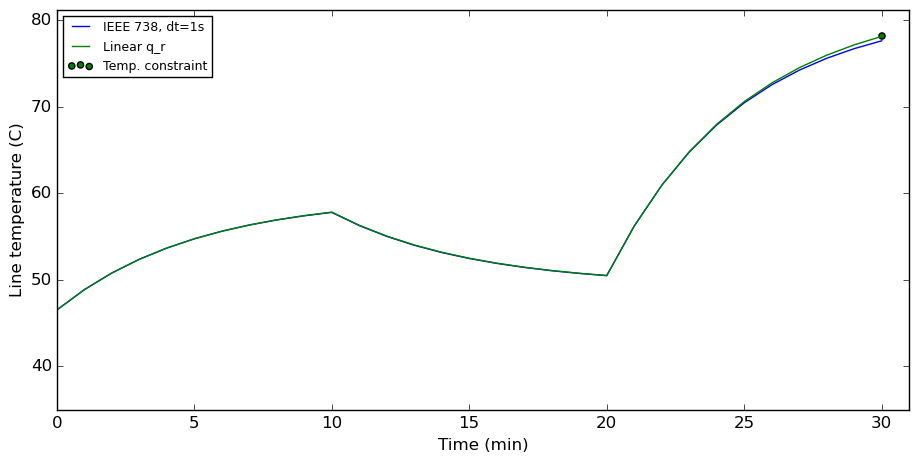
\includegraphics[width=1\linewidth]{../images/temp_model_comparison2}
\caption{Comparison of IEEE 738 and approximate temperature calculation methods}
\label{fig:temp_model_comparison2}
\end{figure}

The blue trace in Figure \ref{fig:temp_model_comparison2} results from numerical integration of \eqref{eq:738heatbalance} with a 1s step size. The green trace comes from the approximate model derived in Section \ref{transmission-line-heating}. The green dot is the final temperature computed by \eqref{eq:almostthere}.

Notes:

\begin{itemize}
\item
  Because the approximate line temperature model is analytic (Equation \eqref{eq:tivp} is continuous) while the 738 model requires numerical integration, I chose
  a very small integration step size of one second to facilitate comparison.
\item
  Because the approximate model underestimates the radiative heat loss
  rate (see Figure \ref{fig:rad_approx}), the green trace should lie slightly above the blue one. This
  makes the approximate model conservative, which is desirable in the
  temporal instanton setting. Figure \ref{fig:temp_model_comparison2} illustrates this conservative behavior: the green trace lies on or above the blue trace throughout the time horizon.
  \item The green dot, computed by \eqref{eq:almostthere}, lies on top of the green curve. This validates the temperature constraint formulation \eqref{eq:tempconstraint}.
\end{itemize}

\section{Conclusion}

An approximate line temperature equation was derived. This equation assumes radiation is linear (not fourth-order) in temperature. There is close numerical agreement between this approximate equation and IEEE 738 standard temperature calculation. The greatest benefit of the approximate temperature equation is that it may be rearranged into a second-order angle difference constraint, which is a requirement of the temporal instanton optimization framework.
    
\end{document}
